\documentclass[11pt]{article}

\usepackage[T1]{fontenc}
\usepackage[polish]{babel}
\usepackage[utf8]{inputenc}
\usepackage{listings}
\usepackage{xcolor}
\usepackage{indentfirst}
\usepackage{graphicx}

\graphicspath{ {../plots/} }

\topmargin=-0.45in
\evensidemargin=0in
\oddsidemargin=0in
\textwidth=6.5in
\textheight=9.0in
\headsep=0.25in

\definecolor{codegreen}{rgb}{0,0.6,0}
\definecolor{codegray}{rgb}{0.5,0.5,0.5}
\definecolor{codepurple}{rgb}{0.58,0,0.82}
\definecolor{backcolour}{HTML}{F2F2F2}

\lstdefinestyle{mystyle}{
    backgroundcolor=\color{backcolour},   
    commentstyle=\color{codegreen},
    keywordstyle=\color{magenta},
    numberstyle=\tiny\color{codegray},
    stringstyle=\color{codepurple},
    basicstyle=\ttfamily\footnotesize,
    breakatwhitespace=false,         
    breaklines=true,                 
    captionpos=b,                    
    keepspaces=true,                 
    numbers=left,                    
    numbersep=5pt,                  
    showspaces=false,                
    showstringspaces=false,
    showtabs=false,                  
    tabsize=4
}

\lstset{style=mystyle}

\title{Projekt WdAD}
\author{Filip Cebula 151410}
\date{\today}

\begin{document}

\maketitle
\pagebreak

\section{Zadanie 1}
\subsection{Podpunkt A}
Zapisujemy dane do naszego zadania.

\begin{lstlisting}[language=R]
earnings = c(45617,7166,18594,2236,1278,19828,4033,28151,2414,3800);
earnings.sd = 15000;
\end{lstlisting}

Estymujemy średnią z próbki, oraz błąd standardowy (korzystając z danego odchylenia standardowego).

\begin{lstlisting}[language=R]
earnings.mean = mean(earnings);
earnings.se = earnings.sd / sqrt(length(earnings));

# Output
# Earnings mean:  13311.7 
# Earnings standard error:  4743.416 
\end{lstlisting}

Obliczamy przedziały ufności 90\%, przy założeniu rozkładu normalnego próbki.

\begin{lstlisting}[language=R]
earnings.interval1 = 0.1;
earnings.ci1.margin = qnorm(p = (1 - earnings.interval1 / 2)) * earnings.se;
earnings.ci1 = earnings.mean + c(-1,1) * earnings.ci1.margin;

# Output
# "Confidence interval for 0.9 assuming normal distribution:"
# 5509.474 21113.926
\end{lstlisting}

Obliczamy przedziały ufności 95\%, przy założeniu rozkładu normalnego próbki.

\begin{lstlisting}[language=R]
earnings.interval2 = 0.05;
earnings.ci2.margin = qnorm(p = (1 - earnings.interval2 / 2)) * earnings.se;
earnings.ci2 = earnings.mean + c(-1,1) * earnings.ci2.margin;

# Output
# "Confidence interval for 0.95 assuming normal distribution:"
# 4014.775 22608.625
\end{lstlisting}

\pagebreak

\subsection{Podpunkt B}
Odrzucamy dane nam wcześniej odchylenie standardowe i estymujemy nowe odchylenie standardowe,
oraz błąd standardowy na podstawie danej próbki.

\begin{lstlisting}[language=R]
earnings.sd = sd(earnings);
earnings.se = earnings.sd / sqrt(length(earnings));

# Output
# Earnings standard derivation:  14662.04 
# Earnings standard error:  4636.545 
\end{lstlisting}

Używamy rozkładu t Studenta, żeby obliczyć przedziały ufności dla naszej próbki.

Przedział ufności 90\%.

\begin{lstlisting}[language=R]
earnings.interval1 = 0.1;
earnings.ci1.margin = qt(p = (1 - earnings.interval1 / 2),
                         df = length(earnings) - 1) * earnings.se;
earnings.ci1 = earnings.mean + c(-1,1) * earnings.ci1.margin;

# Output
# "Confidence interval for 0.9 assuming Student's t-distribution:"
# 4812.39 21811.01
\end{lstlisting}

Przedział ufności 95\%.

\begin{lstlisting}[language=R]
earnings.interval2 = 0.05;
earnings.ci2.margin = qt(p = (1 - earnings.interval2 / 2),
                         df = length(earnings) - 1) * earnings.se;
earnings.ci2 = earnings.mean + c(-1,1) * earnings.ci2.margin;

# Output
# "Confidence interval for 0.95 assuming Student's t-distribution:"
# 2823.107 23800.293
\end{lstlisting}

\pagebreak

\subsection{Podpunkt C}
Odrzucamy założenie o normalności rozkładu naszej próbki. Możemy użyć histogramu,
oraz wykresu kwantyl-kwantyl, aby sprawdzić jak blisko rozkładu normalnego jest
rozkład naszej próbki.

\begin{figure}[h]
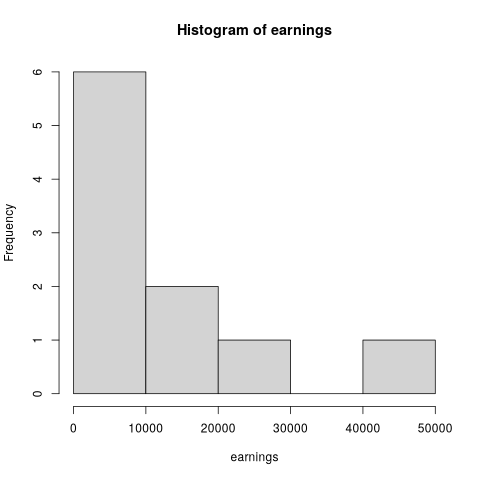
\includegraphics[scale=0.5]{earnings_hist.png}
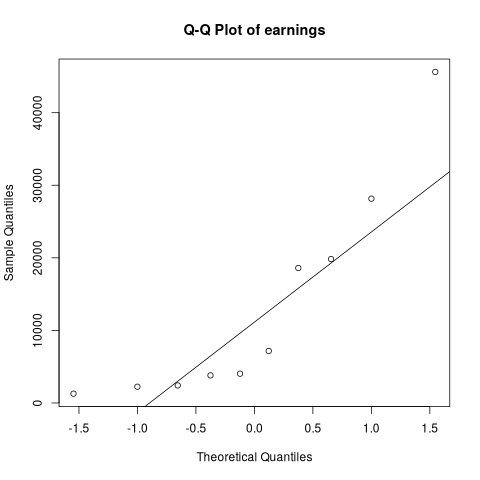
\includegraphics[scale=0.5]{earnings_qq.png}
\centering
\end{figure}

Na podstawie powyższych wykresów, a szczególnie wykresu kwantyl-kwantyl, możemy zauważyć,
że rozkład naszej próbki nie jest rozkładem normalnym. Wynika z tego, że obliczone przez
nas powyżej przedziały ufności nie są dokładne. Aby otrzymać dokładniejsze wyniki, użyjemy
metody bootstrap do obliczenia przedziałów ufności.

\pagebreak

Tworzymy funkcje bootstrap i używamy jej na naszej próbce.

\begin{lstlisting}[language=R]
my_bootstrap = function(data) {
    n = length(data);
    means = c();

    for (i in 1:10000) {
        rands = sample(1:n, n, replace = T);
        xs = data[rands];

        means = append(means, mean(xs));
    }

    return(means);
}

earnings.bootstrap = my_bootstrap(earnings);
\end{lstlisting}

Wyliczamy przedział ufności 90\%.

\begin{lstlisting}[language=R]
quantile(earnings.bootstrap, probs = c(0.05, 0.95));

# Output
# "Confidence interval for 0.9:"
#      5%      95% 
# 6641.84 20903.85 
\end{lstlisting}

Wyliczamy przedział ufności 95\%.

\begin{lstlisting}[language=R]
quantile(earnings.bootstrap, probs = c(0.025, 0.975));

# Output
# "Confidence interval for 0.95:"
#     2.5%     97.5% 
# 5638.485 22847.100 
\end{lstlisting}

\pagebreak

\section{Zadanie 2}
W tym zadaniu do zbadania wybrałem zestawy danych: shrimp, Sitka89 i quine.

Najpierw dodałem bibliotekę MASS, a następnie napisałem drugą metodę bootstrap,
która ułatwi mi liczenie przedziałów ufności dla odchylenia standardowego i wariancji.

\begin{lstlisting}[language=R]
library(MASS);

adv_bootstrap = function(data, f) {
    n = length(data);
    result = c();

    for (i in 1:10000) {
        rands = sample(1:n, n, replace = T);
        xs = data[rands];

        result = append(result, f(xs));
    }

    return(result);
}
\end{lstlisting}

\pagebreak

\subsection{Shrimp}
Shrimp to zestaw danych, który opisuje ilość krewetek (procent całkowitej masy)
w koktajlu krewetkowym.

\begin{figure}[h]
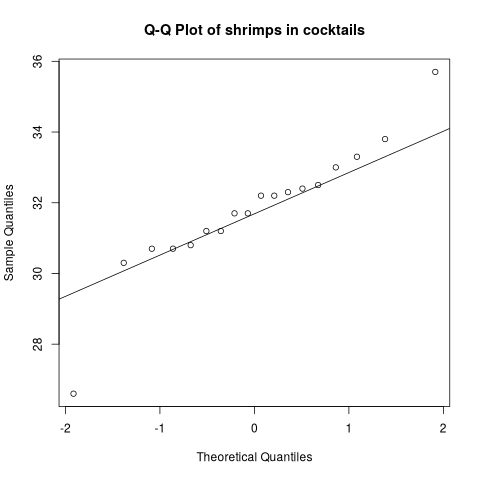
\includegraphics[scale=0.5]{shrimps_qq.png}
\centering
\end{figure}

Na powyższym wykresie możemy zauważyć, że poza dwoma wartościami skrajnymi,
rozkład naszych danych jest bardzo zbliżony do rozkładu normalnego, jednak
o ciężkich ogonach (fat tails), co oznacza zbyt dużą kurtozę.

Obliczmy zatem przedziały ufności 95\%, dla średniej, odchylenia standardowego i wariancji.

\begin{lstlisting}[language=R]
shrimps.bootstrap.mean = adv_bootstrap(shrimp, mean);
shrimps.bootstrap.sd = adv_bootstrap(shrimp, sd);
shrimps.bootstrap.var = adv_bootstrap(shrimp, var);

# Output
# "Confidence intervals for 0.95 for shrimps:"
# "Mean:"
#    2.5%    97.5% 
# 30.92222 32.57222 
# "Standard deviation:"
#     2.5%     97.5% 
# 0.8732765 2.5980592 
# "Standard error:"
#     2.5%     97.5% 
# 0.7527917 6.7226168 
\end{lstlisting}

\pagebreak

\subsection{Npk}
Npk to zestaw danych z eksperymentu, który testował wpływ azotu, fosforu i potasu
na wzrost groszku. Ja skupiłem się na statystyce yield, która zawiera infromacje
o tym, ile grochu zebrano na jednej działce.

\begin{figure}[h]
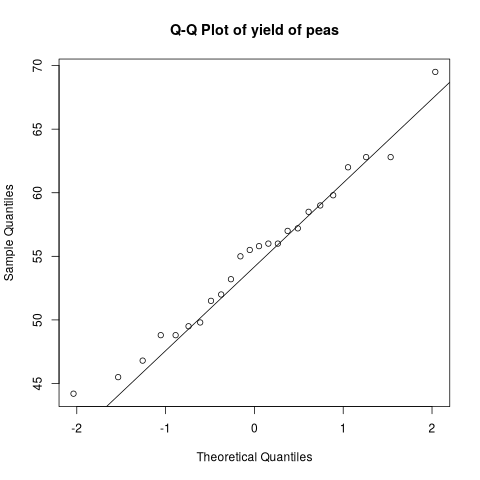
\includegraphics[scale=0.5]{npkyield_qq.png}
\centering
\end{figure}

Na powyższym wykresie widzimy, że rozkład naszych danych, jest bardzo podobny do
rozkładu normalnego. Jednak nasz rozkład ba bardzo lekkie ogony, co oznacza ujemną
kurtozę.

Obliczmy zatem przedziały ufności 95\%, dla średniej, odchylenia standardowego i wariancji.

\begin{lstlisting}[language=R]
npkyield.bootstrap.mean = adv_bootstrap(npk$yield, mean);
npkyield.bootstrap.sd = adv_bootstrap(npk$yield, sd);
npkyield.bootstrap.var = adv_bootstrap(npk$yield, var);

# Output
# "Confidence intervals for 0.95 for npk yield:"
# "Mean:"
#   2.5%   97.5% 
# 52.4625 57.3500 
# "Standard deviation:"
#    2.5%    97.5% 
# 4.422683 7.627811 
# "Standard error:"
#    2.5%    97.5% 
# 19.73285 57.91169 
\end{lstlisting}

\pagebreak

\subsection{Quine}
Quine to zestaw danych, który zawiera informacje o uczniach z Austalii. Ja skupiłem
się na statystyce, która przedstawi ile dni dane dziecko opuściło w trakcie roku szkolnego.

\begin{figure}[h]
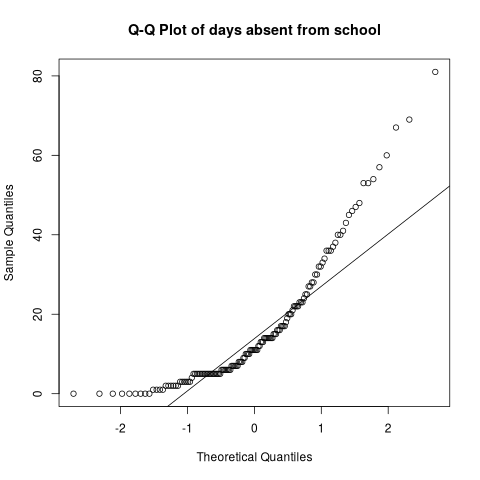
\includegraphics[scale=0.5]{quineabsent_qq.png}
\centering
\end{figure}

Na powyższym wykresie możemy zauważyć, że nasz rozkład znacząco odbiega od
rozkładu normalnego, ponieważ nasz rozkład jest zbyt pozytywnie skośny (tj. 
pochyla się na lewą stonę).

Obliczmy zatem przedziały ufności 95\%, dla średniej, odchylenia standardowego i wariancji.

\begin{lstlisting}[language=R]
quineabsent.bootstrap.mean = adv_bootstrap(quine$Days, mean);
quineabsent.bootstrap.sd = adv_bootstrap(quine$Days, sd);
quineabsent.bootstrap.var = adv_bootstrap(quine$Days, var);

# Output
# "Confidence intervals for 0.95 for absent days:"
# "Mean:"
#    2.5%    97.5% 
# 13.96575 19.13031 
# "Standard deviation:"
#    2.5%    97.5% 
# 13.43493 18.74195 
# "Standard error:"
#    2.5%    97.5% 
# 181.1858 353.6281 
\end{lstlisting}

\end{document}
